%%%%%%%%%%%%%%%%%%%%%%%%%% lecture-10
%\begin{frame}[shrink]
%  \frametitle{lecture-10 主要内容}
%  \framesubtitle{二维数组和字符数组}
%  \tableofcontents[hideallsubsections]
%\end{frame}



\section{定义和引用二维数组: int a[10][20];}

\begin{frame}[shrink,fragile]{二维数组应用场景}
\vspace{-0.3cm}
\begin{example}
	有3个小分队,每队有6名队员,要把这些队员的工资用数组保存起来以备查。
	\begin{tabular}{|c|c|c|c|c|c|c|}
		\hline 
	     & \textcolor{blue}{队员1} & \textcolor{blue}{队员2} & \textcolor{blue}{队员3} & \textcolor{blue}{队员4} & \textcolor{blue}{队员5} & \textcolor{blue}{队员6}\\
	    \hline  
	    \textcolor{blue}{第1分队}& 1000 & 2000 & 1500 & 2400 & 3000 & 5000\\ 
		\hline 
		\textcolor{blue}{第2分队}& 3000 & 4000 & 2500 & 2300 & 2500 & 4000\\ 
		\hline 
		\textcolor{blue}{第3分队}& 4000 & 5000 & 1200 & 2300 & 3200 & 5500\\ 
		\hline 
	\end{tabular} 
\end{example}
\begin{lstlisting}
float pay[3][6]; // 定义3行6列的二维数组, 称为3x6矩阵(matrix)。
\end{lstlisting}
\begin{tabular}{c|c|c|c|c|c|c|}
	\cline{2-7}  
	1分队 & pay[0][0] & pay[0][1] & pay[0][2] & pay[0][3] & pay[0][4] & pay[0][5] \\ 
	\cline{2-7}   
	2分队& pay[1][0] & pay[1][1] & pay[1][2] & pay[1][3] & pay[1][4] & pay[1][5] \\ 
	\cline{2-7}   
	3分队 & pay[2][0] & pay[2][1] & pay[2][2] & pay[2][3] & pay[2][4] & pay[2][5] \\ 
	\cline{2-7}  
\end{tabular} 
\end{frame}

\begin{frame}[shrink,fragile]{定义二维数组: int a[10][20];}
定义二维数组: \\
\textcolor{blue}{元素类型\quad 数组名[行数][列数]}
\begin{lstlisting}
int a[5][10]; // 定义5行10列的整型二维数组,边界:a[0][0],a[4][9]
float pay[3][6]; // 定义3行6列的单精度浮点型二维数组
double pay1[3][6]; // 定义3行6列的双精度浮点型二维数组
char c[2][20]; // 定义2行20列的字符型二维数组

// 好的定义, 行数列数定义为常量, 易控制数组的边界。
#define M 5  // 估计最大行数
#define N 10 // 估计最大列数
int a[M][N]; // 定义M行N列的整型二维数组, 边界:a[0][0],a[M-1][N-1]
\end{lstlisting}
\end{frame}

\begin{frame}[shrink,fragile]{二维数组的存储}
\begin{columns}
\column{0.8\textwidth}
\begin{lstlisting}
float a[3][4]; // 定义3行4列的单精度浮点型二维数组
\end{lstlisting}
\vspace{-0.3cm}
\begin{block}{Notes}
	\small
	用矩阵形式(如3行4列形式)表示二维数组,是逻辑上的概念,能形象地表示出行列关系。而在内存中,各元素是连续存放的,不是二维的,是线性的。\\
	数组元素的下标从0开始,int a[3][4]; 12个整型元素,先行后列存储数组元素。右图左列是数组元素在内存中的``虚拟''地址。
\end{block}
\begin{tabular}{|c|c|c|c|c}
	\hline  
	a[0][0] & a[0][1] & a[0][2] & a[0][3] &$\Leftarrow$第0行\\ 
	\hline 
	a[1][0] & a[1][1] & a[1][2] & a[1][3] &$\Leftarrow$第1行\\ 
	\hline 
	a[2][0] & a[2][1] & a[2][2] & a[2][3] &$\Leftarrow$第2行\\ 
	\hline 
\end{tabular} 
\column{0.2\textwidth}
\small
\begin{tabular}{|c|c|}
	\hline  
	1000 & a[0][0] \\ 
	\hline 
	1004 & a[0][1] \\ 
	\hline 
    1008 & a[0][2] \\ 
	\hline 
	1012 & a[0][3] \\ 
	\hline 
	1016 & a[1][0] \\ 
	\hline 
	1020 & a[1][1] \\ 
	\hline 
	1024 & a[1][2] \\ 
	\hline 
	1028 & a[1][3] \\ 
	\hline 
	1032 & a[2][0] \\ 
	\hline 
	1036 & a[2][1] \\ 
	\hline 
	1040 & a[2][2] \\ 
	\hline 
	1044 & a[2][3] \\ 
	\hline
\end{tabular} 
\end{columns}
\end{frame}

\section{引用数组: int i=0,j=0; a[i][j]}

\begin{frame}[shrink,fragile]{引用数组: int i=0,j=0; a[i][j]}
\vspace{-0.3cm}
\begin{lstlisting}
#define M 5  // 行数
#define N 10 // 列数
float a[M][N]; // 定义M行N列的单精度浮点型二维数组
int i,j;
a[0][0]=10;  // 给第0行第0列元素赋值
a[M-1][N-1]=20; // 给第M-1行第N-1列元素赋值
\end{lstlisting}
\vspace{-0.2cm}
\begin{columns}[T]
\column{0.5\textwidth}
\begin{lstlisting}[frame=single]
// 数组元素赋值
for(i=0;i<M;i++) //遍历第i行
  for(j=0;j<N;j++) //遍历第j列 
    a[i][j]=i*j; //给第i行第j列元素赋值
    
// 键盘输入数组元素
for(i=0;i<M;i++) // 行
   for(j=0;j<N;j++) // 列
     scanf("%f", &a[i][j]);
\end{lstlisting}
\column{0.42\textwidth}
\begin{lstlisting}[frame=single]
// 输出数组元素
for(i=0;i<M;i++) // 行
   for(j=0;j<N;j++) // 列
   {
      printf("%d\t",a[i][j]);
      if(j==N-1) printf("\n");
   }
\end{lstlisting}
\end{columns}
\vspace{0.1cm}
\end{frame}

\begin{frame}[shrink,fragile]{输出每个小分队的平均工资}
\begin{tikzpicture}
\node[text width=1.0\textwidth] (left) {
\vspace{-0.3cm}
\begin{lstlisting}
#define M 100 // 估计最大的行数
#define N 100 // 估计最大的列数
float pay[M][N]; //按照最大值定义数组的大小
int m,n,i,j; //m,n表示实际pay数组行数和列数
float sum; //每个小分队所有人员的工资总和
scanf("%d%d",&m,&n); // 输入小分队数和队员数, 就是pay数组的实际行数和列数
for(i=0;i<m;i++)  // 依次输入每个队员的工资
	for(j=0;j<n;j++) scanf("%f", &pay[i][j]); // 注意取地址符'&'
for(i=0;i<m;i++) // 行
{
	sum=0; // 内层循环执行前, 必须置零。易忘记!!!
	for(j=0;j<n;j++) // 列
		sum += pay[i][j]; // 累加第i小分队所有人员的工资
	printf("第%d小分队平均工资=%f\n",i+1,sum/n);
}
\end{lstlisting}
};
\node[anchor=north west] at($(left.north east)+(-7.5,0)$) {
\tiny
\begin{tabular}{c|c|c|c|c|c|c|}
	\cline{2-7}   
	1分队 & pay[0][0] & pay[0][1] & pay[0][2] & pay[0][3] & pay[0][4] & pay[0][5] \\ 
	\cline{2-7}  
	2分队 & pay[1][0] & pay[1][1] & pay[1][2] & pay[1][3] & pay[1][4] & pay[1][5] \\ 
	\cline{2-7}  
	3分队 & pay[2][0] & pay[2][1] & pay[2][2] & pay[2][3] & pay[2][4] & pay[2][5] \\ 
	\cline{2-7}   
\end{tabular}
};
\end{tikzpicture}
%\vspace{0.01cm}
\end{frame}

\section{二维数组的初始化: int a[2][3]=\{\{1,2,3\},\{4,5,6\},\{7,8,9\} \}}

\begin{frame}[shrink,fragile]{二维数组的初始化: int a[2][3]=\{\{1,2,3\},\{4,5,6\},\{7,8,9\} \}}
\begin{lstlisting}
#define M 3 // 行数
#define N 3 // 列数
int a[M][N]={{1,2,3},{4,5,6},{7,8,9}}; // 定义二维数组, 并初始化
int b[M][N]={{1,2},{4,5},{7,8}}; // 定义二维数组, 并初始化
int c[M][N]={{1,2},{},{7,8}}; // 定义二维数组, 并初始化
// 给未初始化的元素赋值
b[0][N-1]=3;  b[1][N-1]=6; b[2][N-1]=9;
c[0][N-1]=3; 
c[1][0]=4;  c[1][1]=5; c[1][N-1]=6; 
c[2][N-1]=9;
// 利用循环结构,给各元素赋值
int i,j;
for(i=0;i<M;i++)
	for(j=0;j<N;j++)
		a[i][j]=0;
\end{lstlisting}
\end{frame}

\begin{frame}[shrink,fragile]{例6.4 将二维数组行列互换, 存到另一个二维数组中。}
\vspace{-0.4cm}
\small
\[
a=\left[
\begin{array}[c]{ccc}
1 & 2 & 3\\
4 & 5 & 6
\end{array}
\right]
\implies
b=\left[
\begin{array}[c]{cc}
1 & 4\\
2 & 5\\
3 & 6
\end{array}
\right]
\]
\pause
\vspace{-0.5cm}
\begin{lstlisting}
#define M 2 
#define N 3 
int a[M][N]={{1,2,3},{4,5,6}};
int b[N][M],i,j;
\end{lstlisting}
\vspace{-0.4cm}
\begin{columns}[T]
\column{0.4\textwidth}
\pause
\begin{lstlisting}
for(i=0;i<M;i++) // 行
{
   for(j=0;j<N;j++) // 列
   {
      printf("%5d",a[i][j]);
      b[j][i]=a[i][j]; 
   }
   printf("\n"); // 换行
}
\end{lstlisting}
\column{0.4\textwidth}
\pause
\begin{lstlisting}[frame=leftline]
for(i=0;i<N;i++) // 行
{
   for(j=0;j<M;j++) // 列
   {
     printf("%5d",b[i][j]); 
   }
   printf("\n"); // 换行
}
\end{lstlisting}
\end{columns}
\vspace{0.001cm}
\end{frame}

\begin{frame}[shrink,fragile]{例6.5 求二维数组中的最大元素及其行号和列号。}
\vspace{-0.3cm}
\begin{lstlisting}
#define M 2 
#define N 3 
int a[M][N]={{1,2,3},{4,5,6}},i,j,max,row=0,col=0;
max=a[0][0]; // //先认为a[0][0]最大
for(i=0;i<M;i++)  // 行
{
   for(j=0;j<N;j++) // 列
   {
     if(a[i][j]>max)
     { 
        max=a[i][j]; row=i; col=j;
     } 
   }
}
printf("max=%d,row=%d,col=%d\n",max,row,col);
\end{lstlisting}
\end{frame}

\begin{frame}[shrink,fragile]{\small{例: 使方阵(行数=列数)右对角线元素置1, 其它元素为0.}}
\begin{tikzpicture}[font=\scriptsize]
\matrix (4N) [matrix of nodes,nodes={anchor=north,minimum size=6mm,draw},column 1/.style={red},row 1/.style={red}]
{
	|[draw=none]|$i~\backslash~j$ & |[draw=none]|0  & |[draw=none]|1  & |[draw=none]|2   & |[draw=none]|3 \\
	|[draw=none]|0 & $0,0$ & $0,1$ & $0,2$  & $0,3$ \\
	|[draw=none]|1 & $1,0$  & $1,1$ & $1,2$  & $1,3$ \\
	|[draw=none]|2 & $2,0$  & $2,1$  & $2,2$ & $2,3$ \\
	|[draw=none]|3 & $3,0$  & $3,1$  & $3,2$ & $3,3$ \\
};

\path[-]
(4N-5-2.center) edge[blue] node[pos=1,anchor=south east]{左对角线$i+j=3$} +(45:3.4cm)
(4N-2-2.center) edge[red] node[pos=1,anchor=north east]{右对角线$i=j$} +(-45:3.3cm)
;

\node[draw,right,text width=.33\textwidth] (r) at($(4N.east)+(0.2,0)$) {
\vspace{-0.3cm}
\begin{lstlisting}
#define M 10 
int a[M][M],i,j;
for(i=0;i<M;i++) // 行
{
   for(j=0;j<M;j++) // 列
   {
      if(i==j) a[i][j]=1; 
      else a[i][j]=0;
   }
}
\end{lstlisting}
};

\node[draw,anchor=north west,text width=.38\textwidth] at($(r.north east)$) {
\vspace{-0.3cm}
\begin{lstlisting}
// 输出
for(i=0;i<M;i++) // 行
{
   for(j=0;j<M;j++) // 列
      printf("%5d", a[i][j]); 
   printf("\n"); // 换行
}
\end{lstlisting}

\vspace{1.6cm}
~\\
};
\end{tikzpicture}
\end{frame}

\begin{frame}[fragile]{方阵(行数=列数)的上下三角形}
\begin{tikzpicture}[font=\scriptsize]
\matrix (4N) [matrix of nodes,nodes={anchor=north,minimum size=6mm,draw},column 1/.style={red},row 1/.style={red}]
{
	|[draw=none]|$i~\backslash~j$ & |[draw=none]|0  & |[draw=none]|1  & |[draw=none]|2   & |[draw=none]|3 \\
	|[draw=none]|0 & $0,0$ & $0,1$ & $0,2$  & $0,3$ \\
	|[draw=none]|1 & $1,0$  & $1,1$ & $1,2$  & $1,3$ \\
	|[draw=none]|2 & $2,0$  & $2,1$  & $2,2$ & $2,3$ \\
	|[draw=none]|3 & $3,0$  & $3,1$  & $3,2$ & $3,3$ \\
};

\node[below,align=left] at(4N.south) {下三角形(j<i)\\
上三角形(j>i)\\
对角线(j==i)};

\path[-,thick]
(4N-2-2.center) edge[blue] (4N-5-2.center) 
(4N-5-2.center) edge[blue] (4N-5-5.center) 
(4N-2-2.center) edge[blue] (4N-5-5.center) 
;

\node[draw,right,text width=.6\textwidth] (r) at($(4N.east)+(0.2,0)$) {
	\vspace{-0.3cm}
	\begin{lstlisting}
	#define M 10 
	int a[M][M],i,j;
	for(i=0;i<M;i++) // 行
	{
		for(j=0;j<M;j++) // 列
		{
			//下三角形(含对角线)元素置1
			if(j<=i) a[i][j]=1; 
			else a[i][j]=0;     //上三角形元素置0
		}
	}
	\end{lstlisting}
};

\end{tikzpicture}
\end{frame}

\begin{frame}[shrink,fragile]{\small{例: 使方阵(行数=列数)下三角阵(含对角线)元素置1, 其它元素为0.}}
\vspace{-0.4cm}
\begin{columns}[T]
\column{0.4\textwidth}
\begin{lstlisting}
#define M 10 
int a[M][M],i,j;
for(i=0;i<M;i++) // 行
   for(j=0;j<M;j++) // 列
   {
     //下三角形(含对角线)
     if(j<=i) a[i][j]=1; 
     else a[i][j]=0;
   }
printf("下三角阵\n"); 
for(i=0;i<M;i++) // 行
{
   for(j=0;j<=i;j++) // 列
      printf("%5d", a[i][j]); 
   printf("\n"); // 换行
}
\end{lstlisting}
\column{0.6\textwidth}
\begin{lstlisting}[frame=leftline]
printf("上三角阵\n"); 
for(i=0;i<M;i++) // 行
{
    for(j=0;j<M;j++) // 列
       if(j>=i) printf("%5d", a[i][j]);
       else printf("%5c", ' '); 
    printf("\n"); // 换行
}
\end{lstlisting}
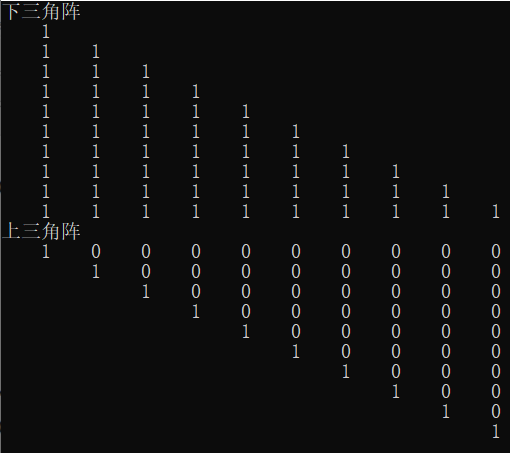
\includegraphics[scale=0.2]{matrix2}
\end{columns}
\vspace{0.001cm}
\end{frame}

\section{用字符数组表示字符串char s[81]}

\begin{frame}[shrink,fragile]{用字符数组表示字符串char s[81]}
字符数组是用来存放字符数据的数组是字符数组。字符数组中的一个元素存放一个字符。\\
~\\
两种方式初始化字符数组
\begin{lstlisting}
// s[0]='a', s='b', s='c', s[3]='d', s[4]以后的字符未赋值
char s[81]={'a','b','c','d'};  // 4个有效字符

// 以'\0'结尾的字符串是C语言表示字符串的标准形式. 
// str[0]='a', str[1]='b', str[2]='c', str[3]='d', str[4]='\0'
// 自动追加'\0', 表示字符串结束. 特别注意, 字符串结尾字符'\0'
char str[]="abcd"; // 5个有效字符
\end{lstlisting}
\end{frame}

\begin{frame}[shrink,fragile]{使用printf函数输出字符串}
\vspace{-0.3cm}
\begin{lstlisting}
// s[0]='a', s='b', s='c', s[3]='d', s[4]以后的字符未赋值
char s[81]={'a','b','c','d'}; // 4个有效字符
for(i=0;i<4;i++)
  printf("%c\t",s[i]); // a b c d

// str[0]='a', str[1]='b', str[2]='c', str[3]='d', str[4]='\0'
// 自动追加'\0', 表示字符串结束
char str[]="abcd"; // 5个有效字符
for(i=0;a[i]!='\0';i++)
  printf("%c\t",str[i]); // a b c d

// 或使用格式描述符%s, 输出以'\0'结尾的字符串
printf("%s\n",str); // abcd, 输出'\0'以前的字符

printf("%s\n",s); // 错误, 由于s不是以'\0'结尾的字符串
s[4]='\0'; // 使字符数组以'\0'结尾, 就可以使用上一句正常输出了
\end{lstlisting}
\end{frame}

\begin{frame}[shrink,fragile]{使用scanf函数输入字符串}
\begin{lstlisting}
char a[81],b[81],c[81];

// 遇空格或回车结束, 自动追加字符串结束字符'\0'
scanf("%s",a); // 注意字符数组前没有取地址符号'&'
// 例如输入: abc回车,则a[0]='a',a[1]='b',a[2]='c',a[3]='\0'
printf("%s\n",a); // abc

// 以空格隔开,输入3个字符串。自动追加字符串结束字符'\0'
scanf("%s%s%s",a,b,c); 
// 例如输入: How are You回车
printf("%s,%s,%s\n",a,b,c); // How,are,You
\end{lstlisting}
\end{frame}

\begin{frame}[shrink,fragile]{推荐使用gets函数和puts函数输入输出字符串}
\begin{lstlisting}
char a[81];  // 定义字符数组的长度要足够大, 以容纳最后一个字符'\0'

// 可以接收带空格的字符串,遇回车结束, 自动追加字符串结束字符'\0'
gets(a);
// 例如输入: ab cd回车

// 遇字符串结束字符'\0', 换行退出
puts(a); // ab cd
\end{lstlisting}
\end{frame}




